\documentclass[../main.tex]{subfiles}
\begin{document}
	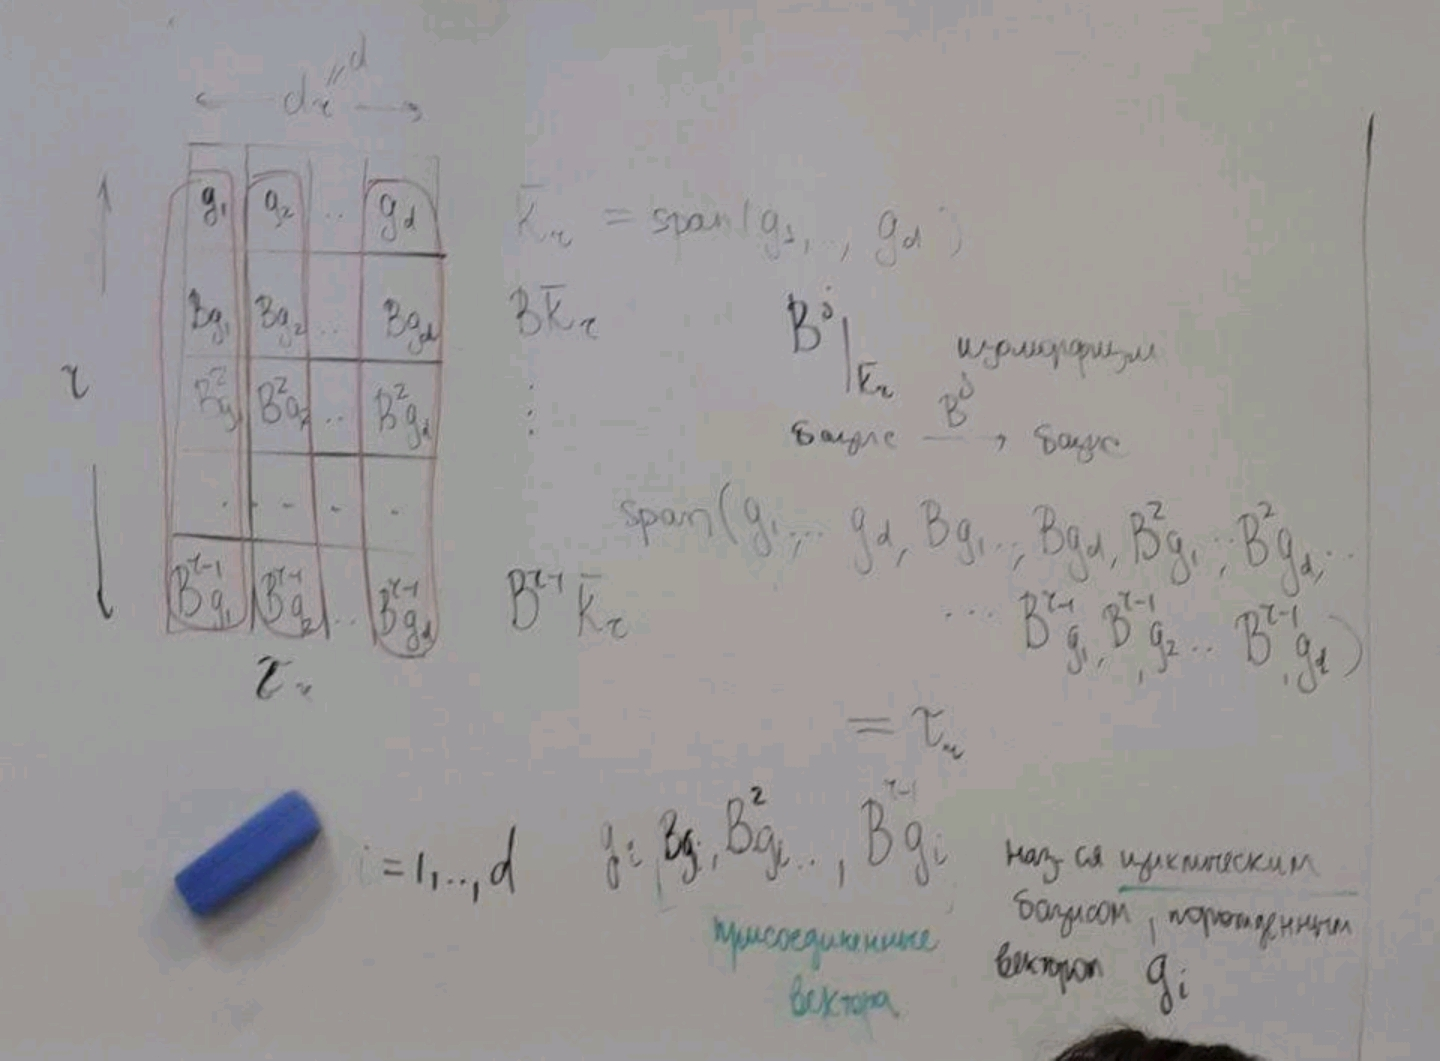
\includegraphics[width=\textwidth]{kek0/kek0_00001}
	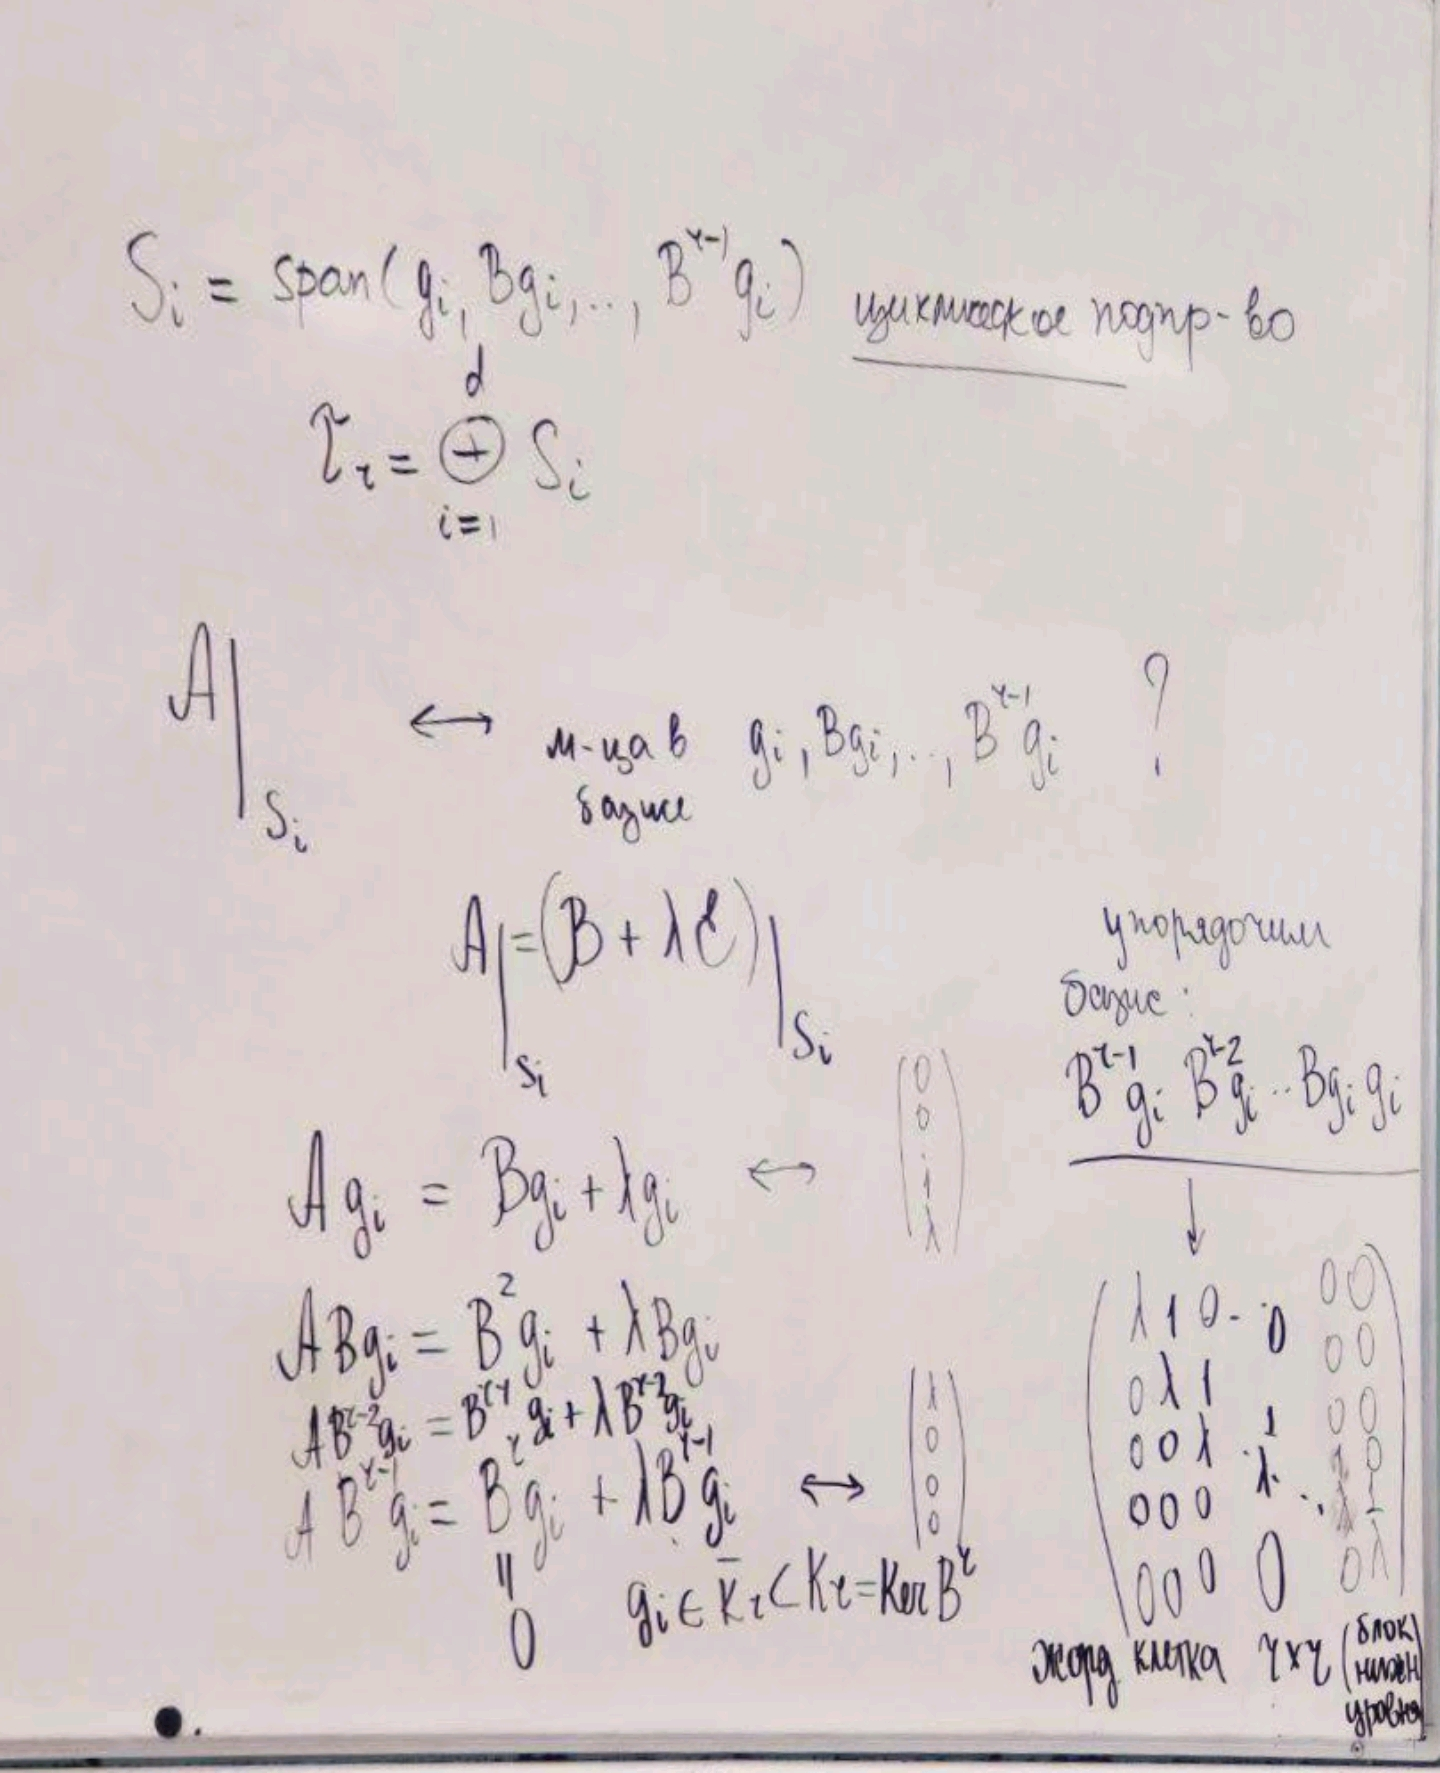
\includegraphics[width=\textwidth]{kek0/kek0_00002}
	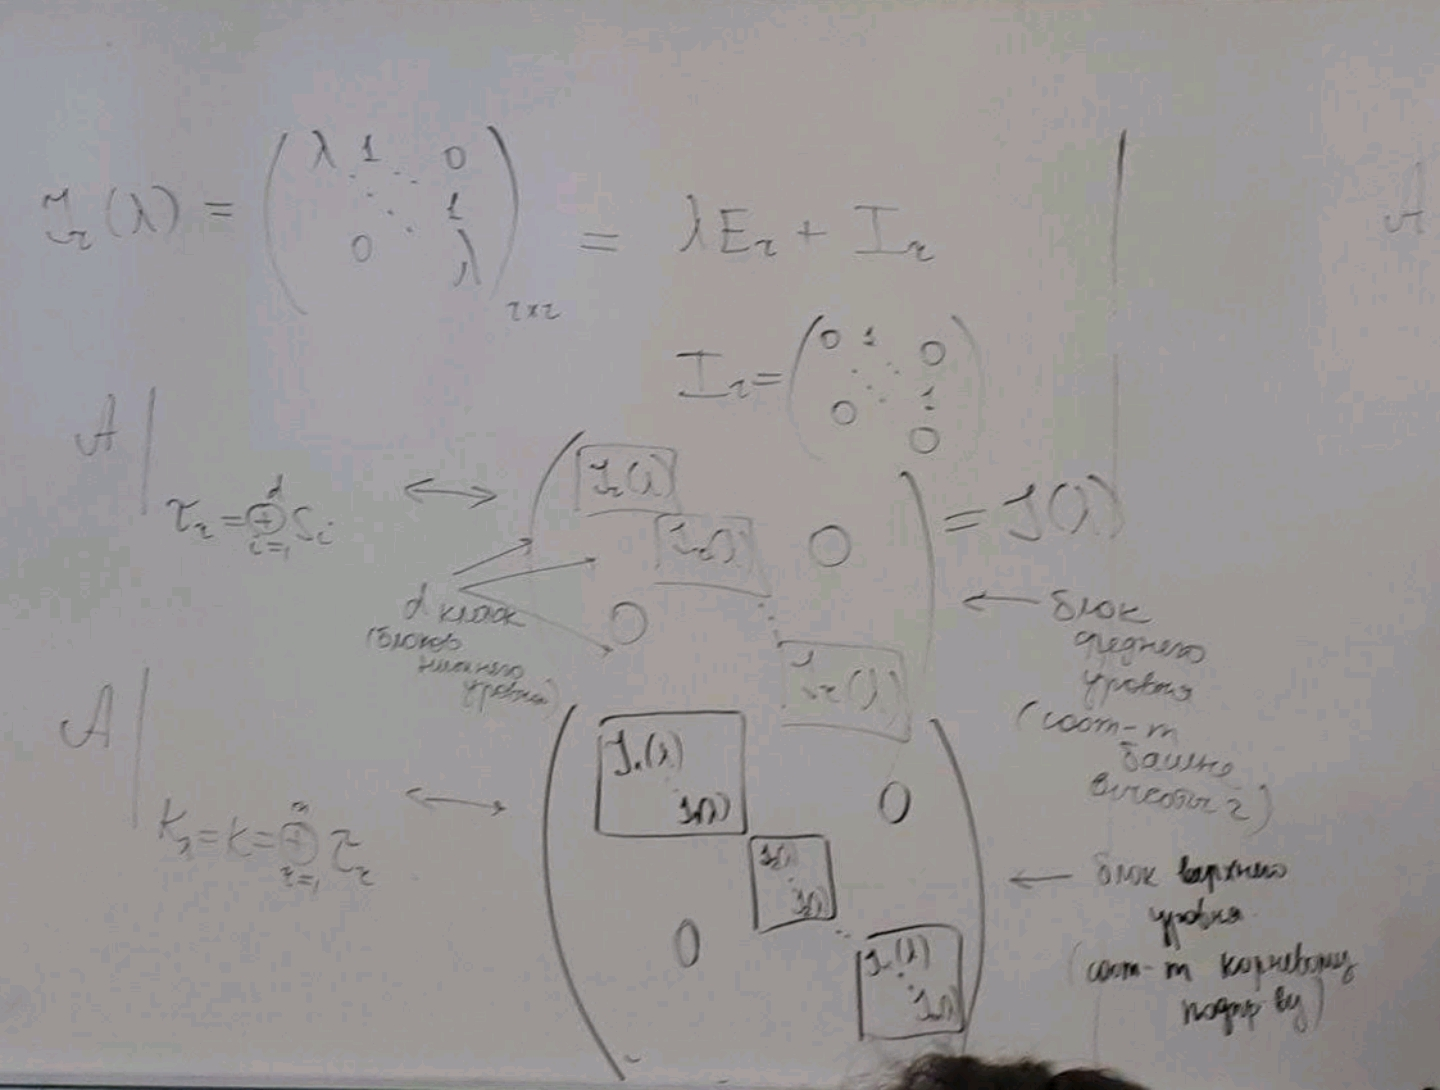
\includegraphics[width=\textwidth]{kek0/kek0_00003}
	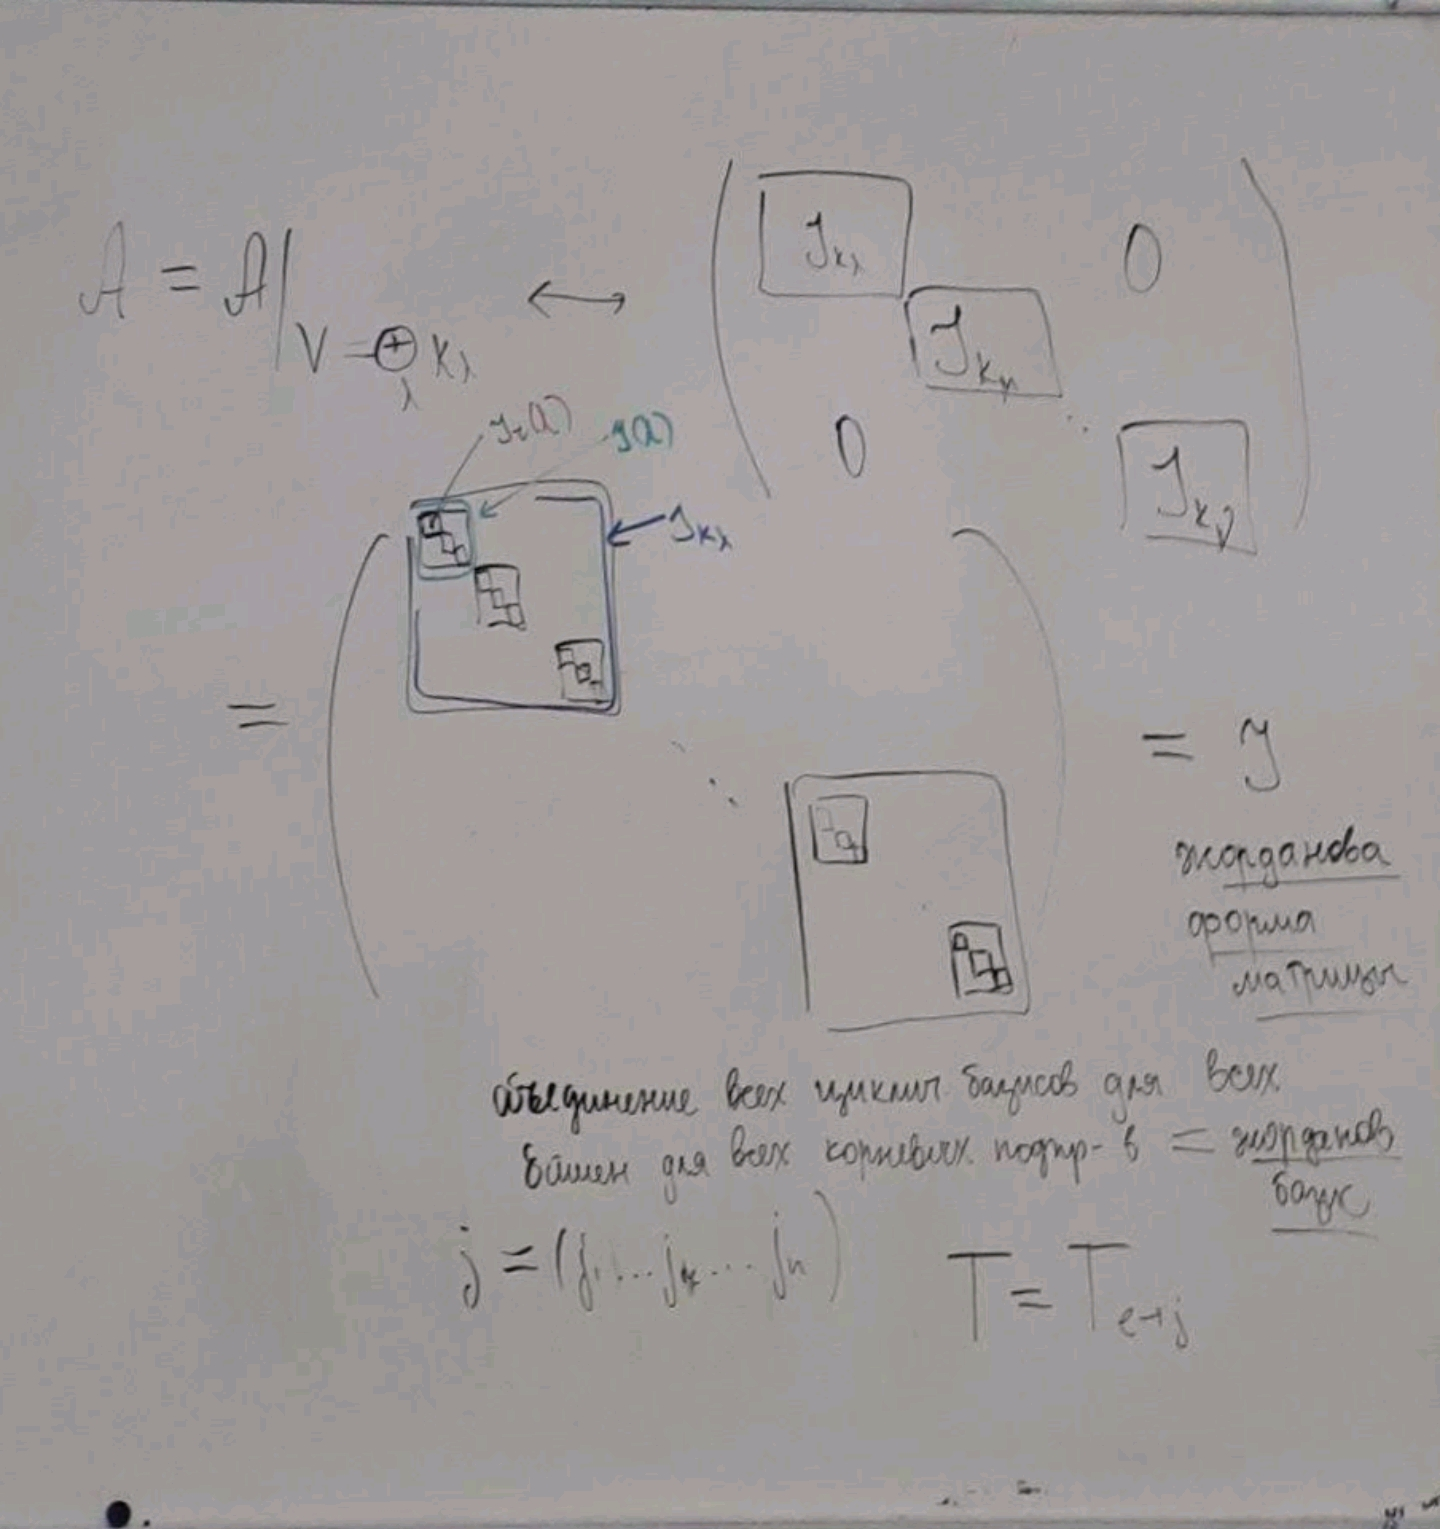
\includegraphics[width=\textwidth]{kek0/kek0_00004}
	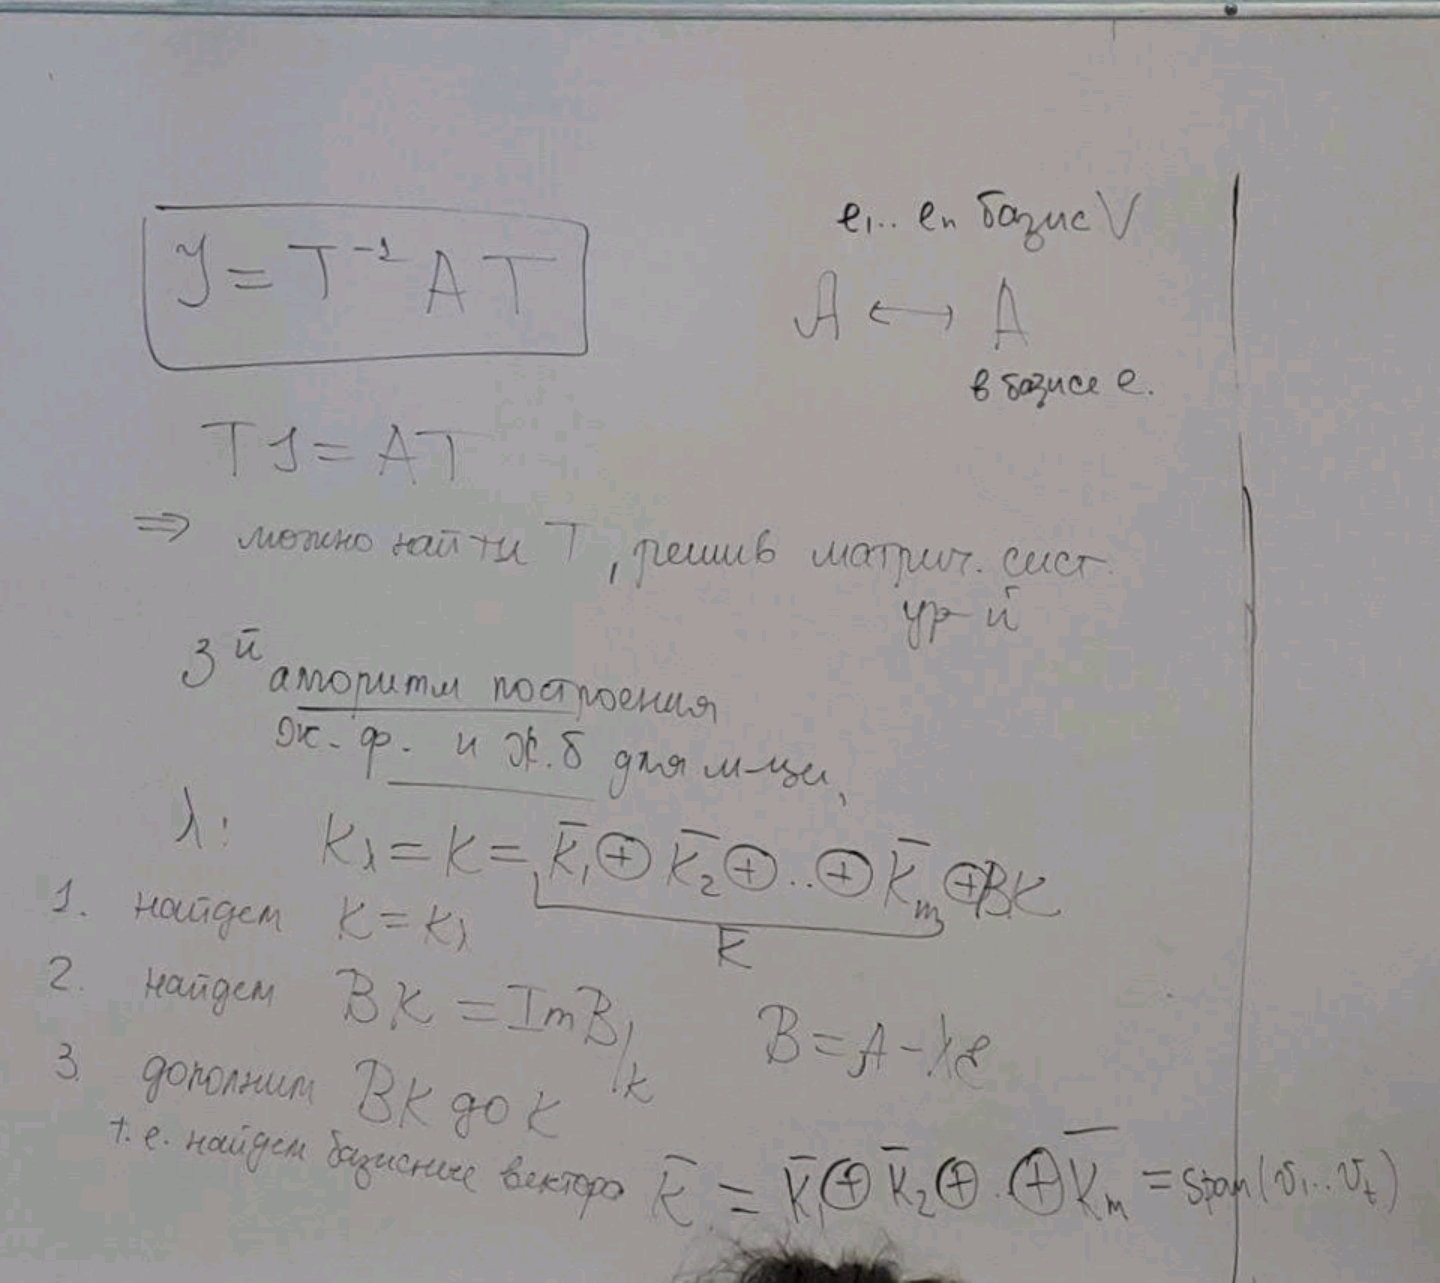
\includegraphics[width=\textwidth]{kek0/kek0_00005}
	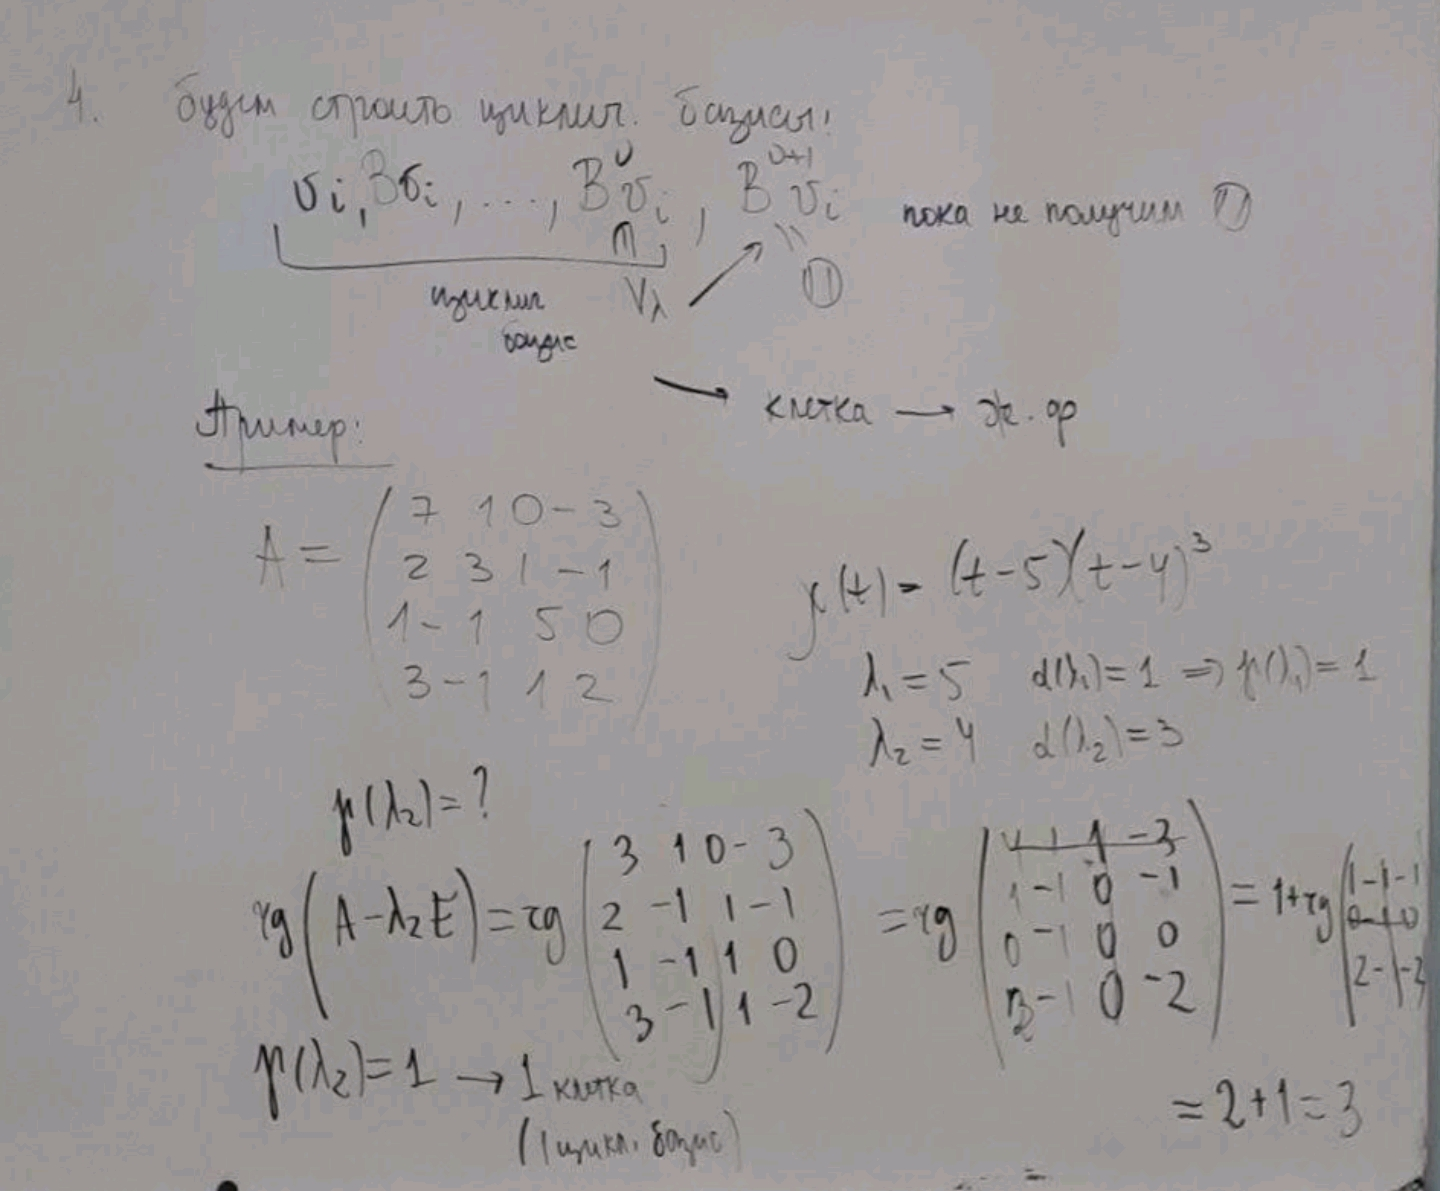
\includegraphics[width=\textwidth]{kek0/kek0_00006}
	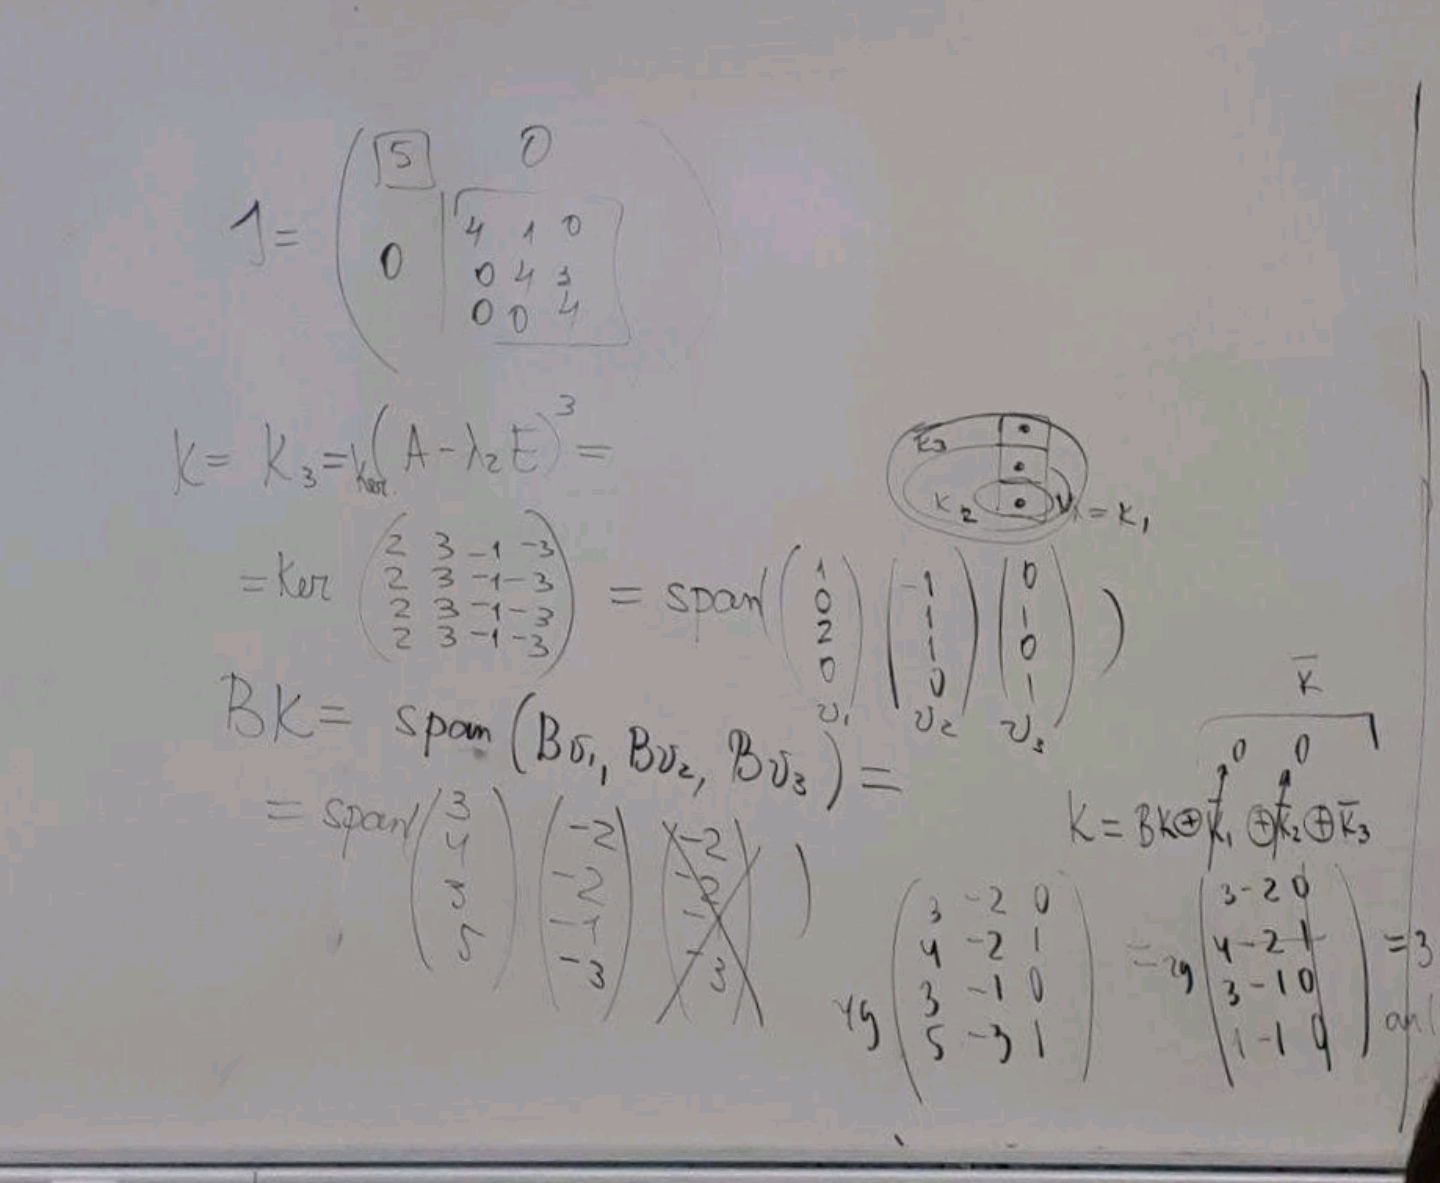
\includegraphics[width=\textwidth]{kek0/kek0_00007}
	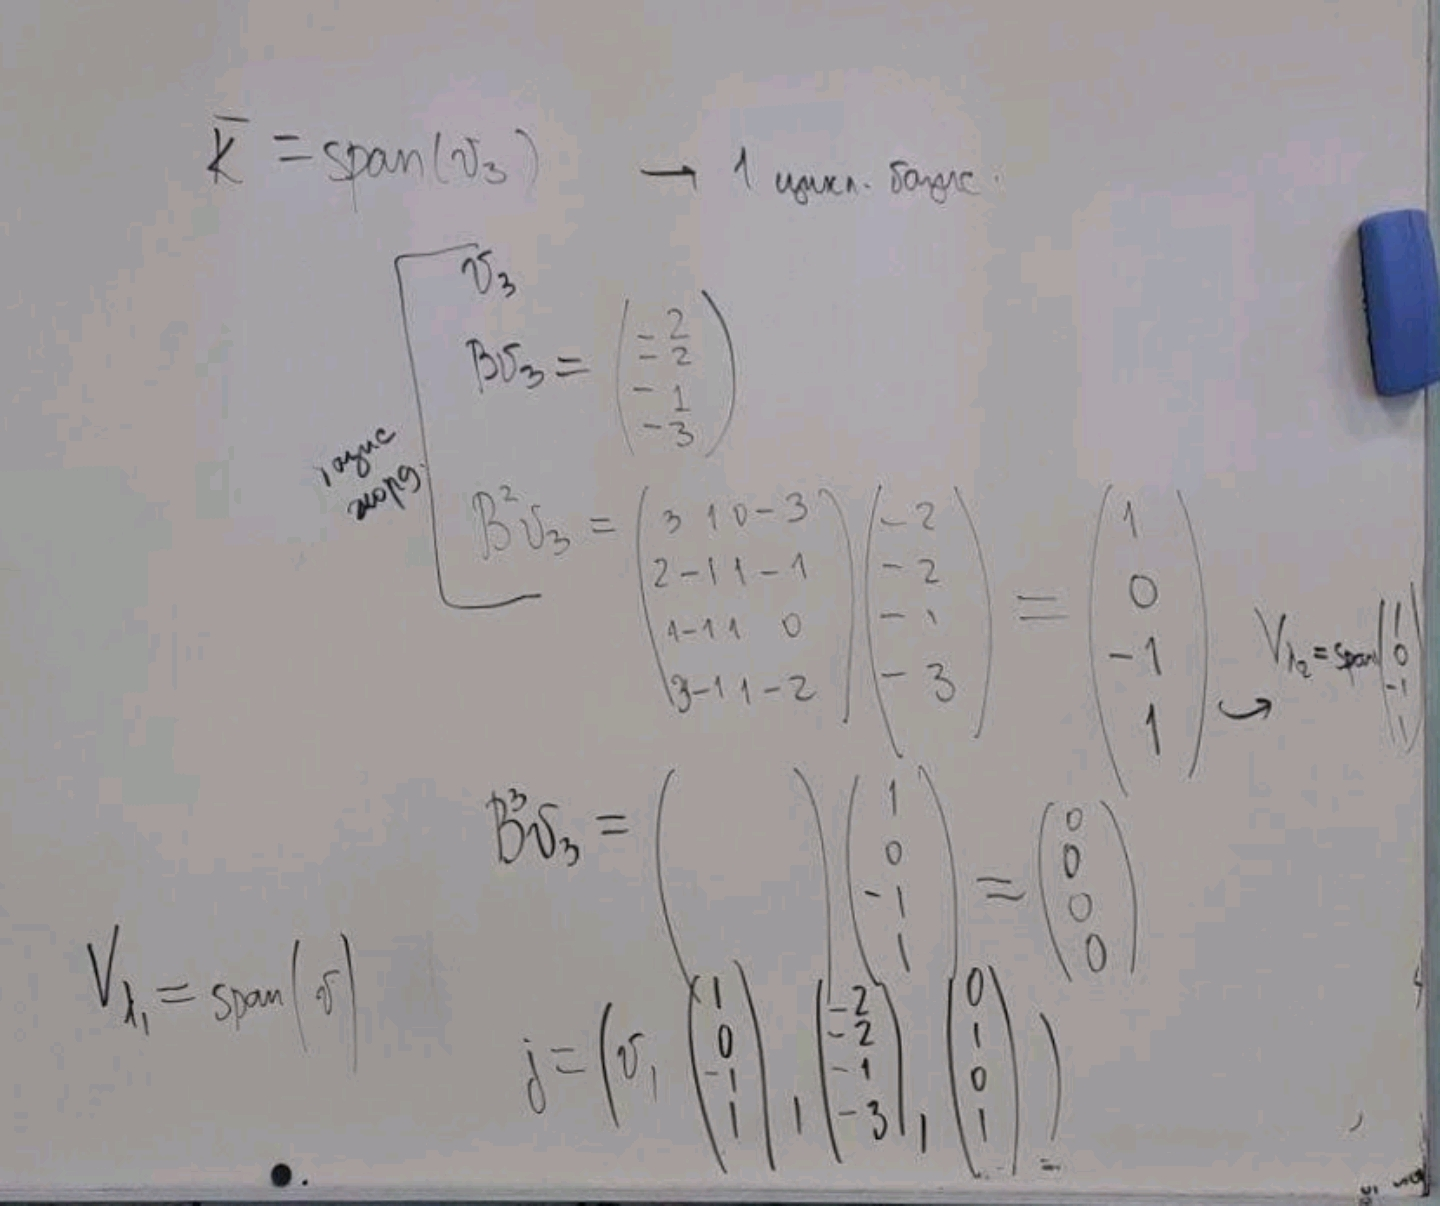
\includegraphics[width=\textwidth]{kek0/kek0_00008}
	\subsection{Функция от матрицы, приведенной к Жордановой форме}
	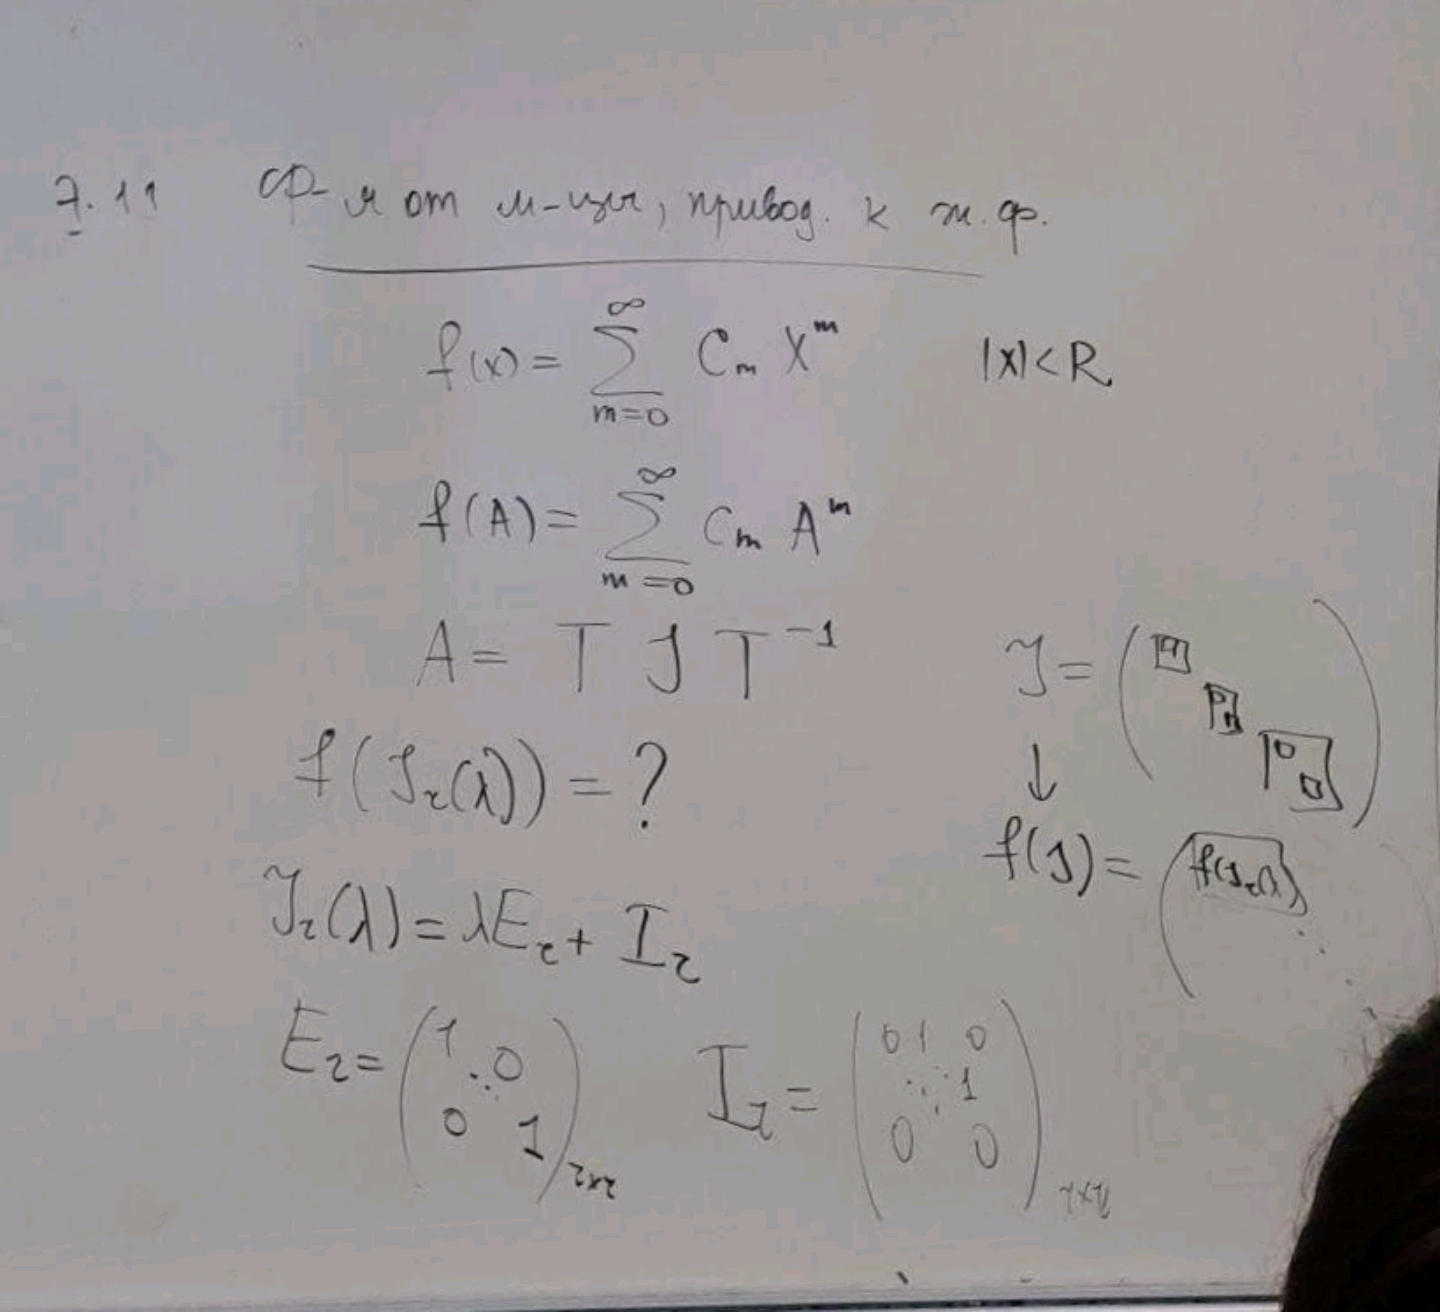
\includegraphics[width=\textwidth]{kek1/kek1_00001}
	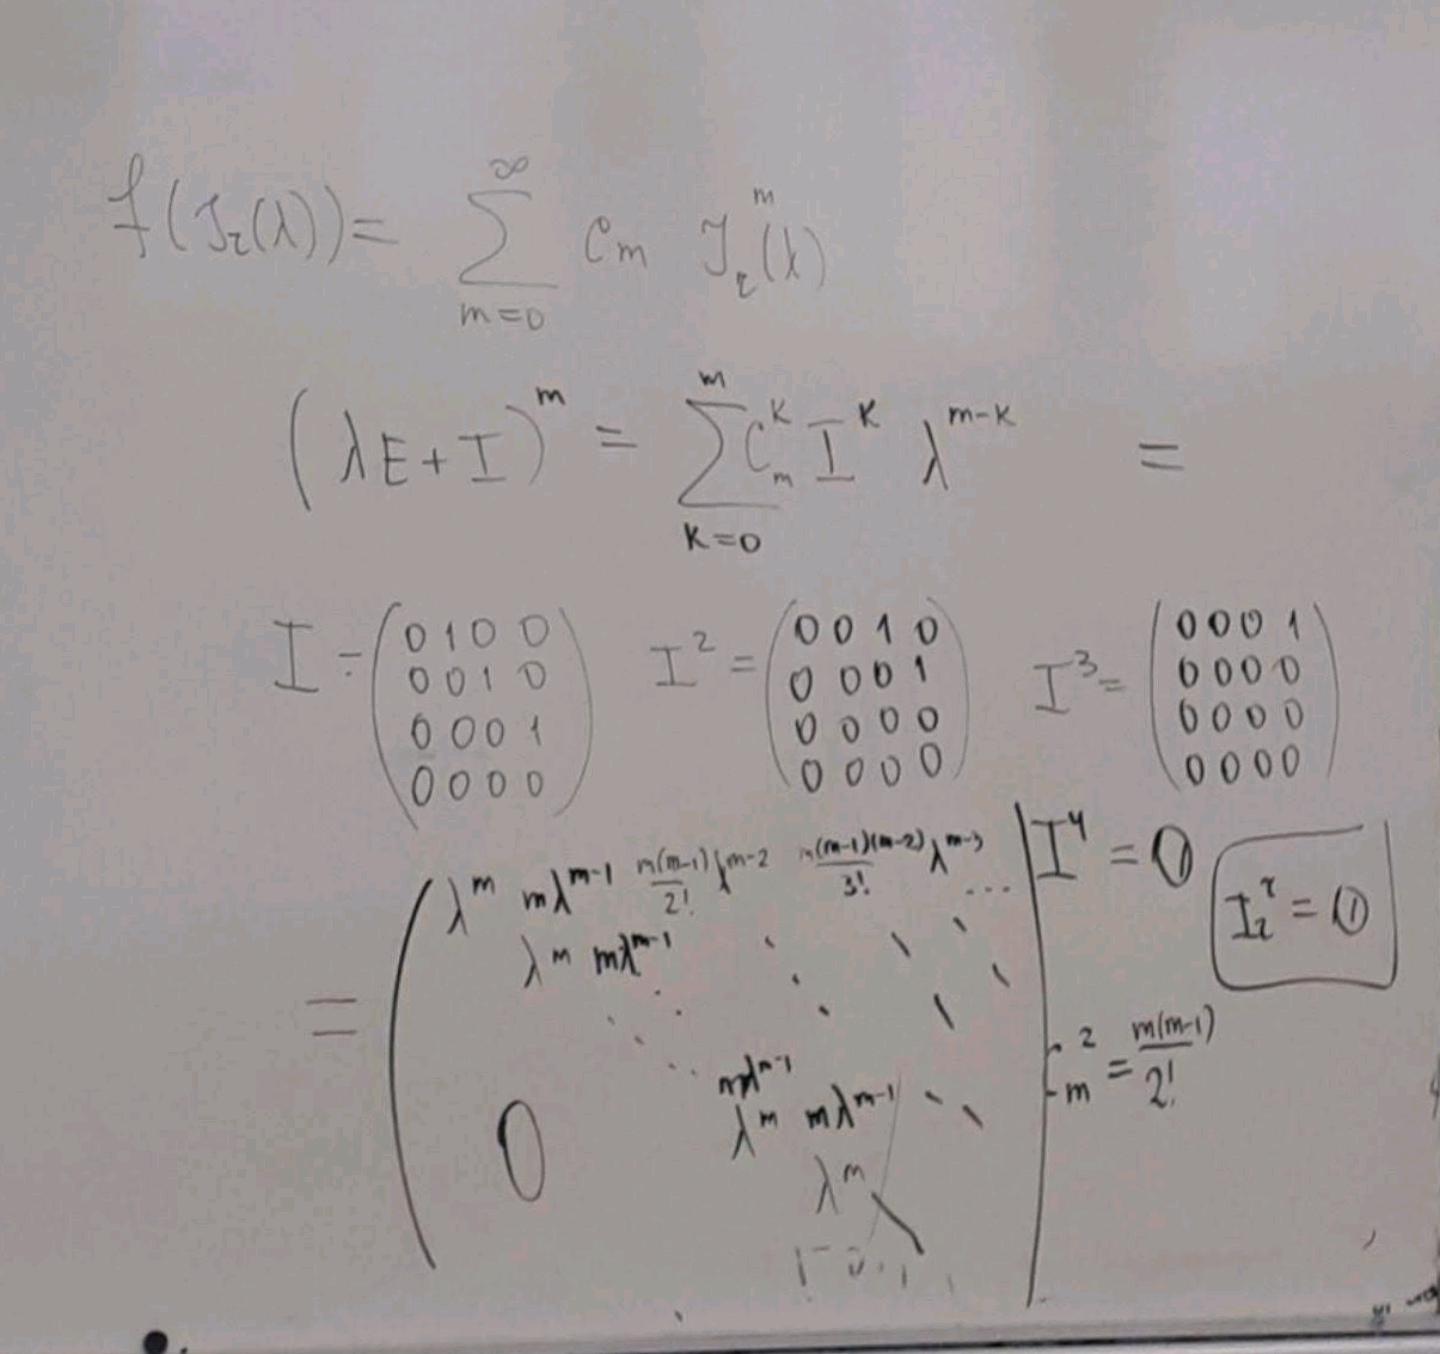
\includegraphics[width=\textwidth]{kek1/kek1_00002}
	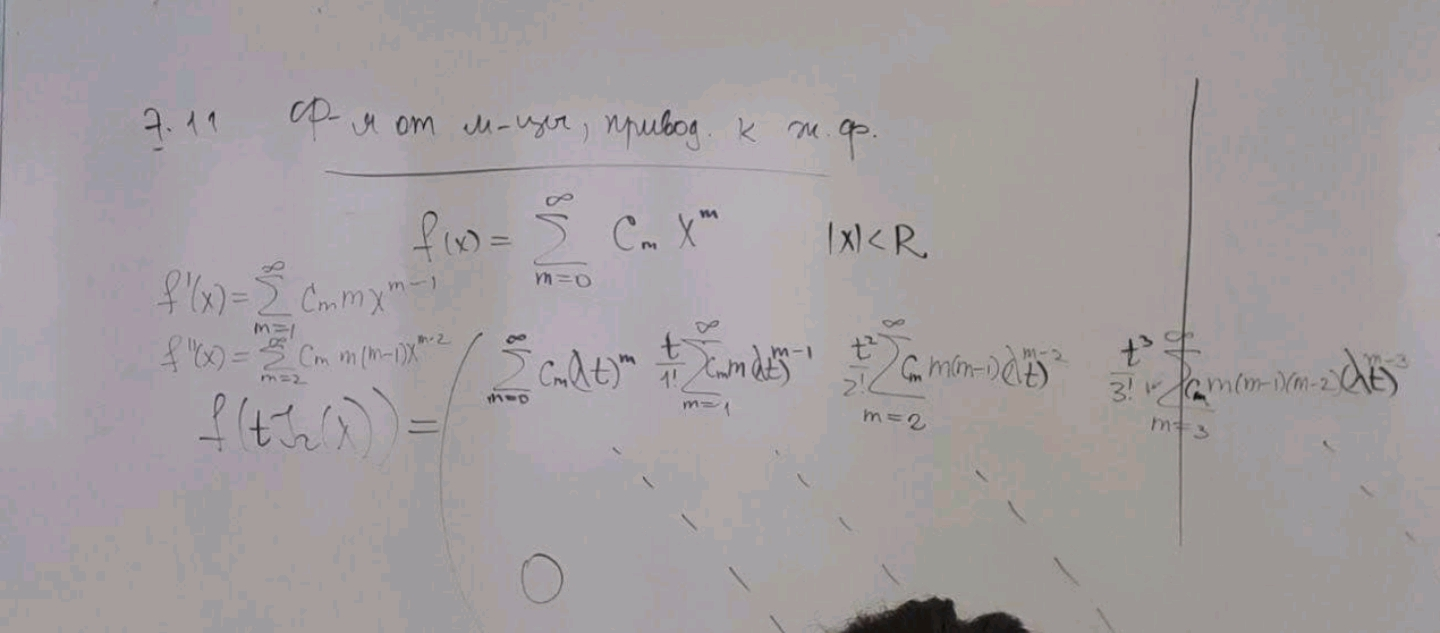
\includegraphics[width=\textwidth]{kek1/kek1_00003}\n
	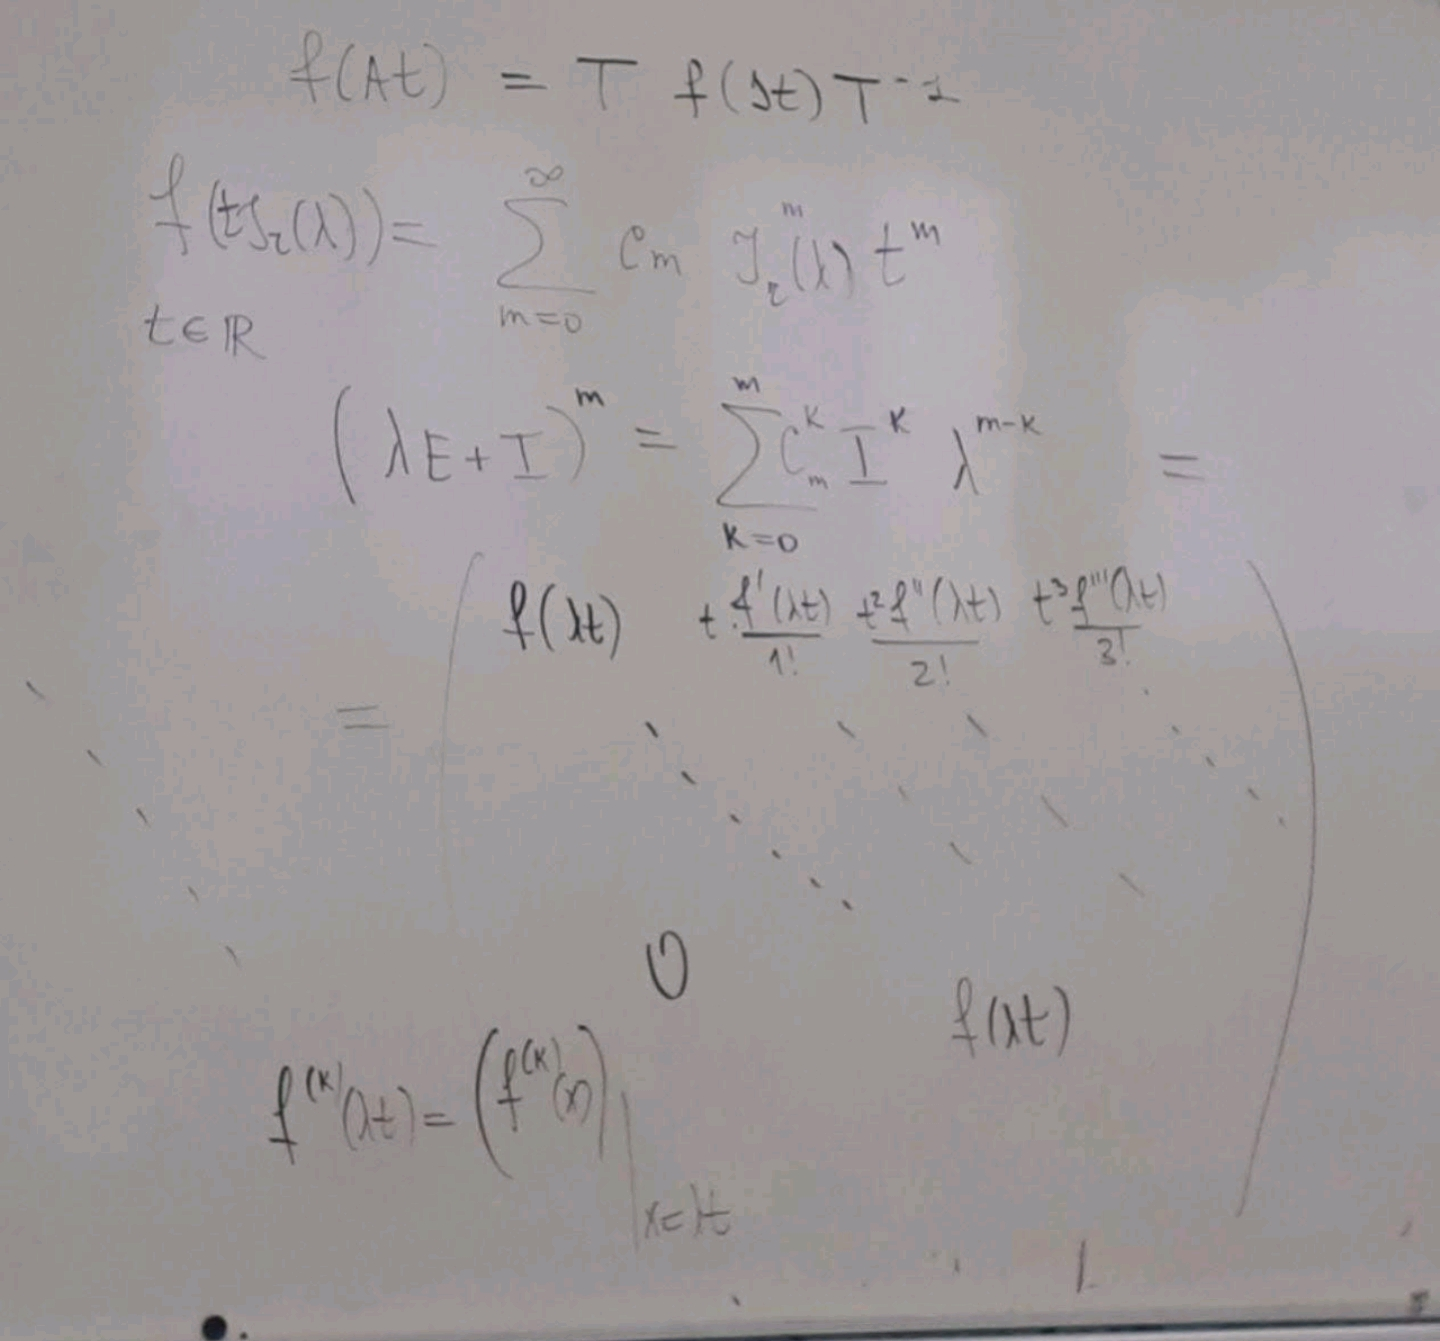
\includegraphics[width=0.9\textwidth]{kek1/kek1_00004}\n
	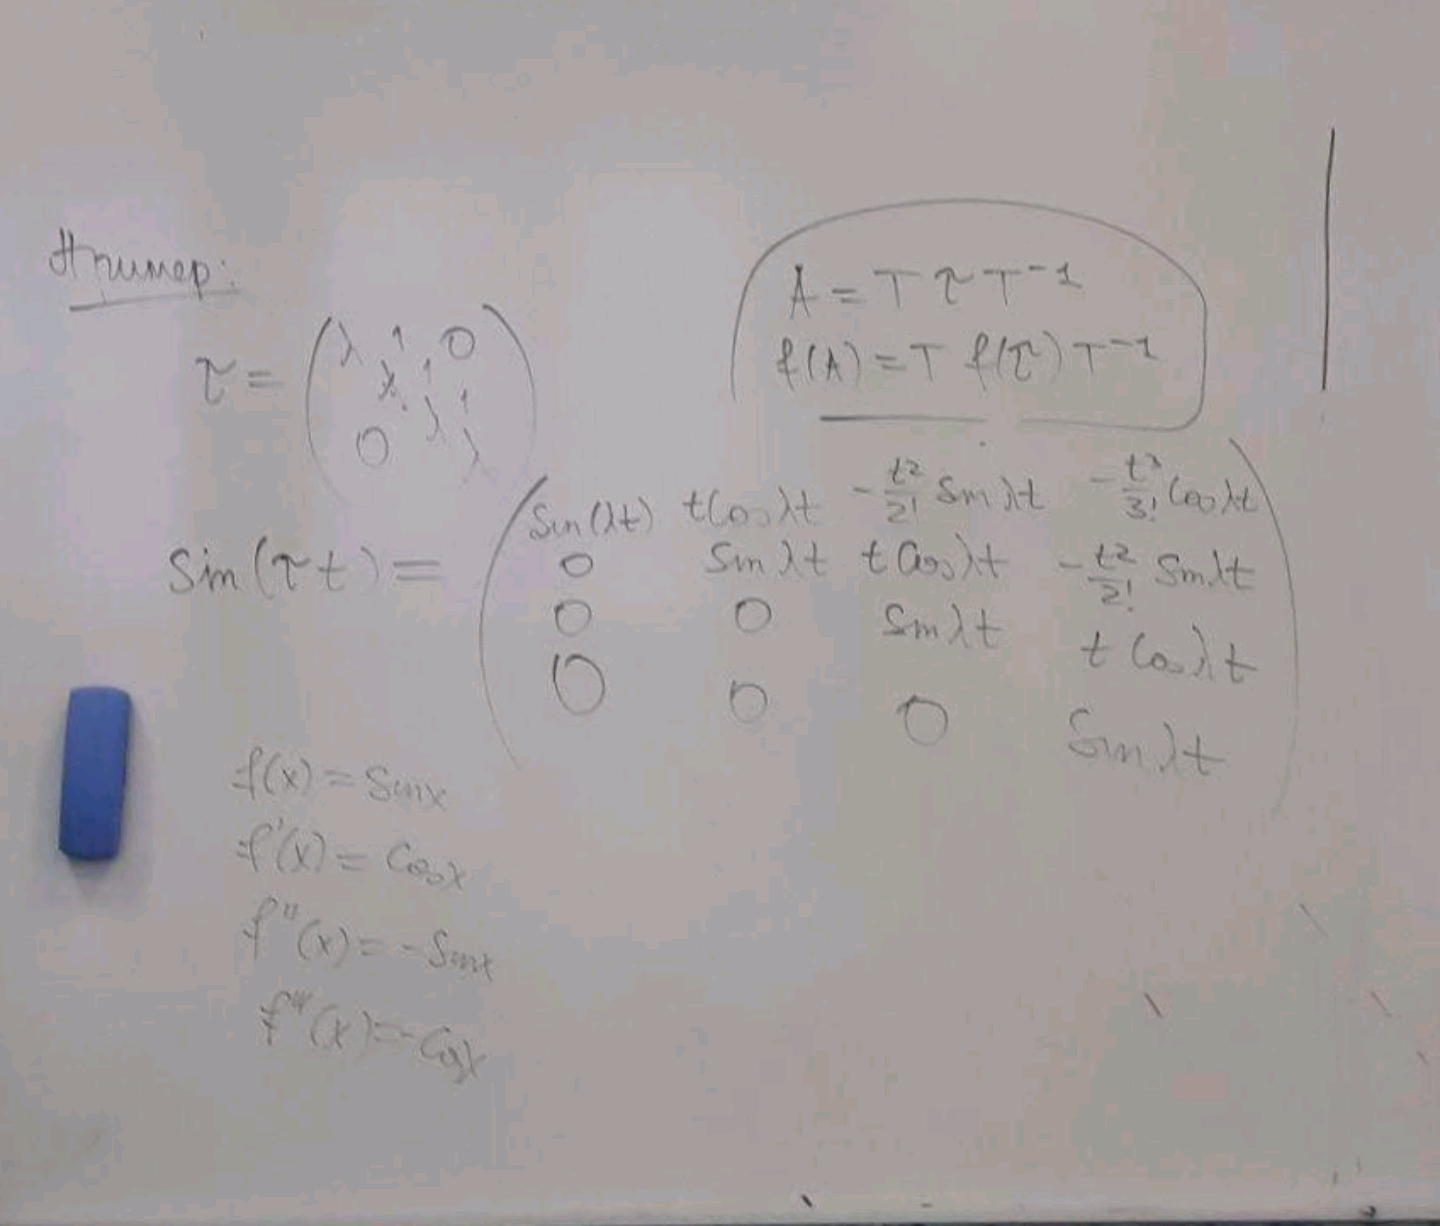
\includegraphics[width=\textwidth]{kek1/kek1_00005}
	\section{Тензоры}
	\subsection{Линейные формы (линейные функционалы). Сопряженное пространство. Ковариантные, 
	контрвариантные преобразования.}
	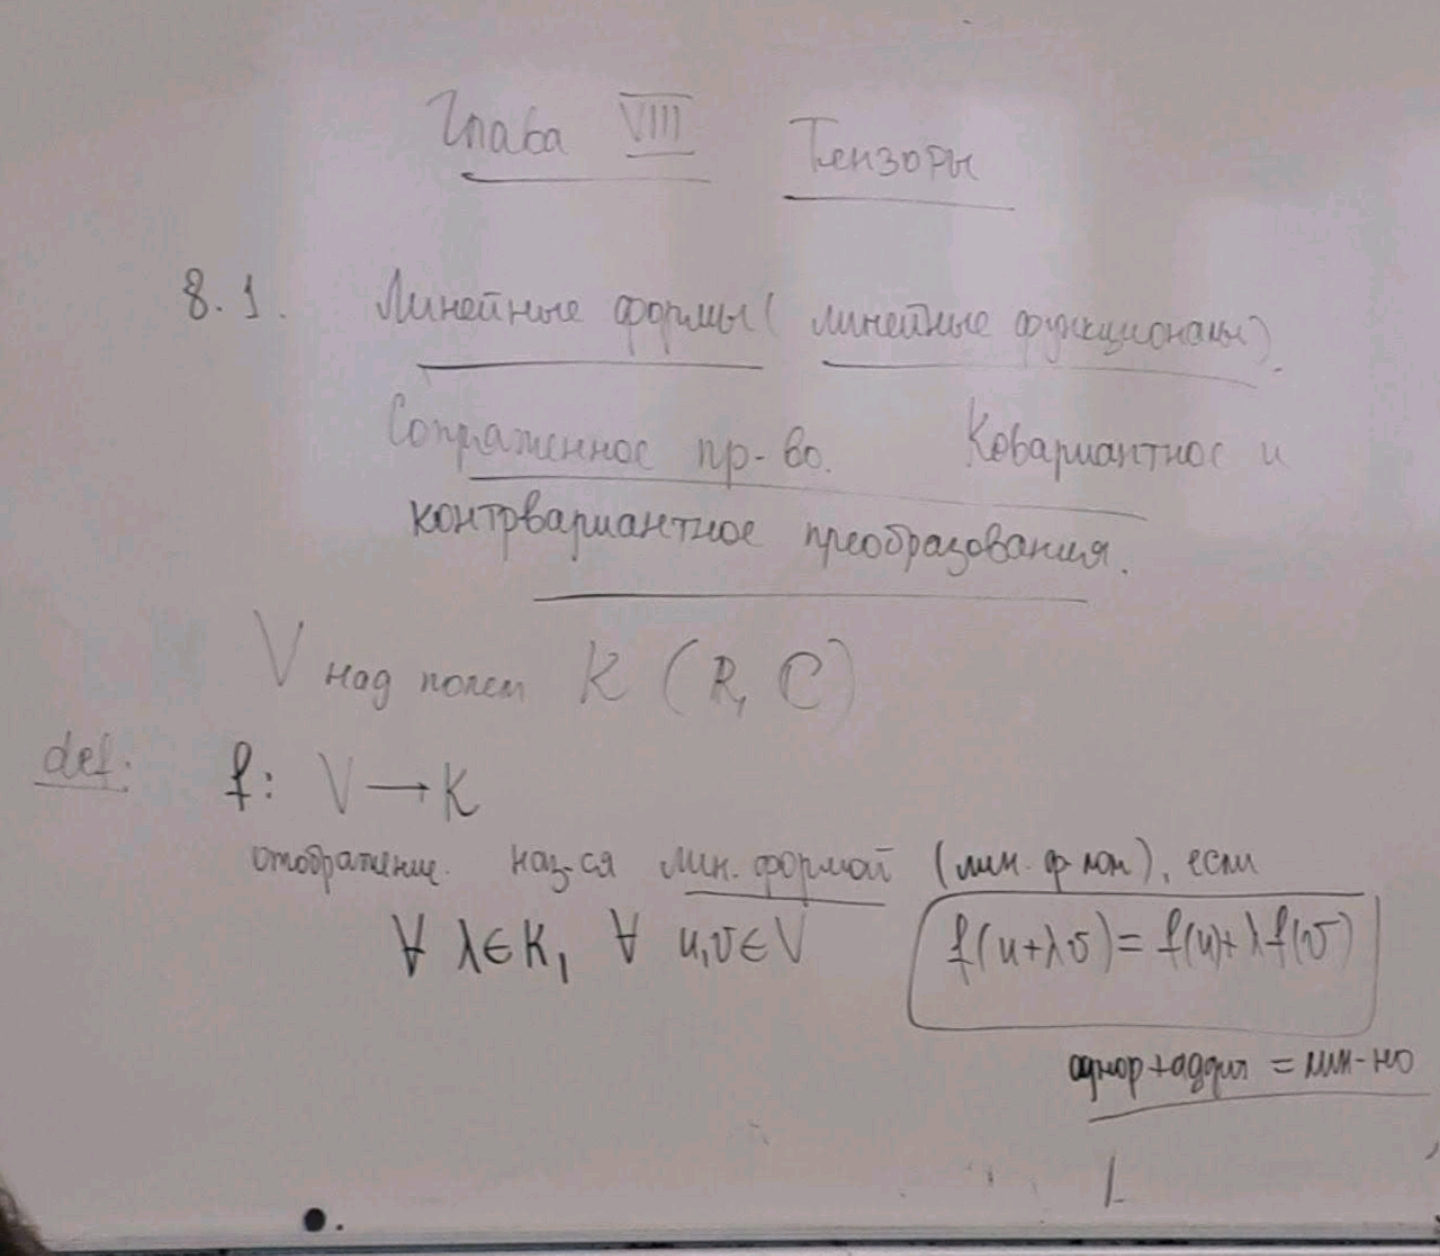
\includegraphics[width=\textwidth]{kek2/kek2_00001}\n
	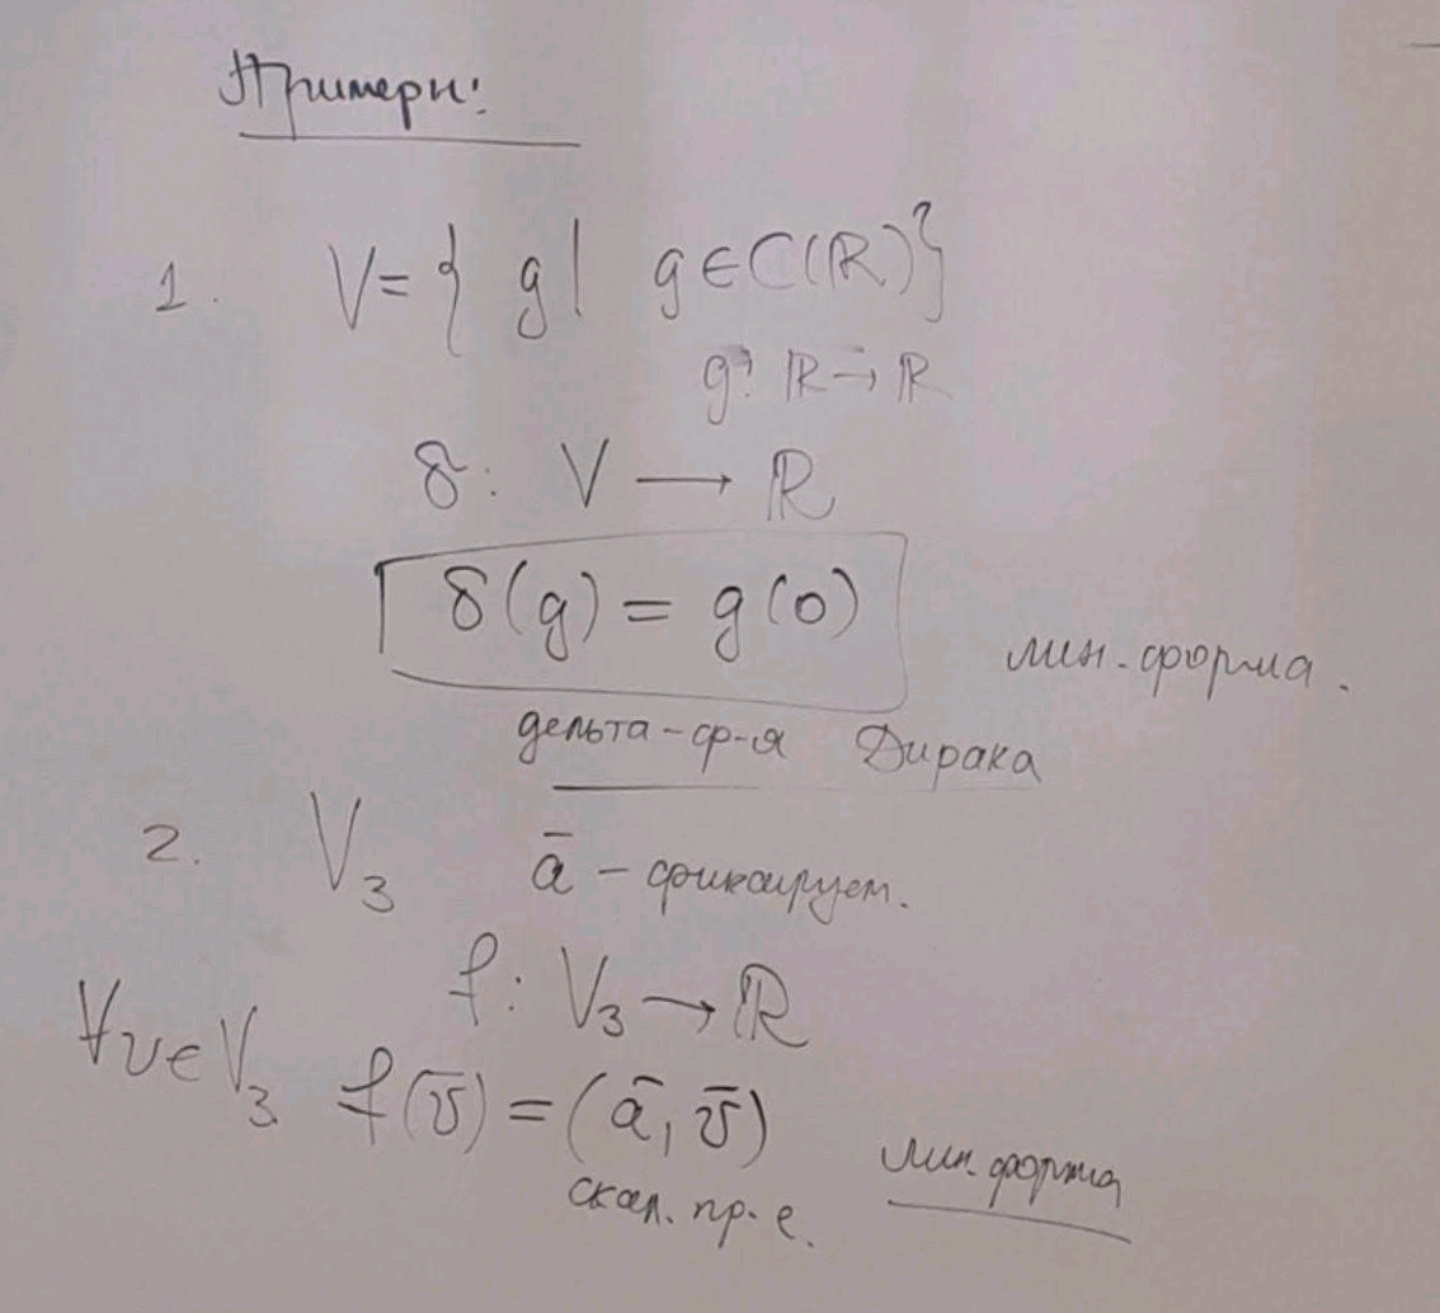
\includegraphics[width=\textwidth]{kek2/kek2_00002}
	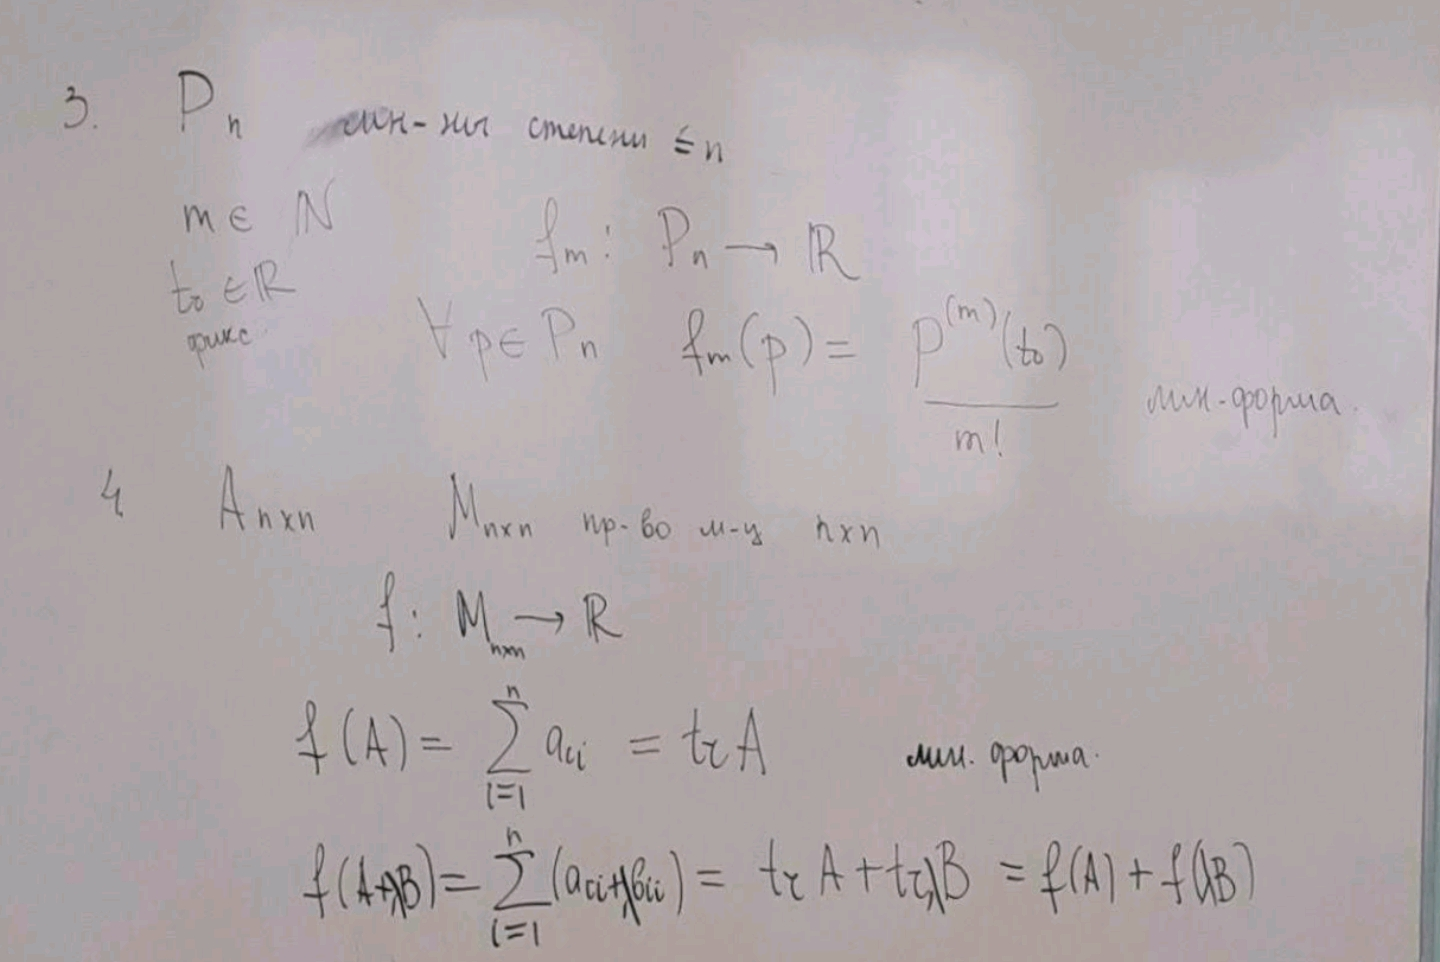
\includegraphics[width=0.93\textwidth]{kek2/kek2_00003}\n
	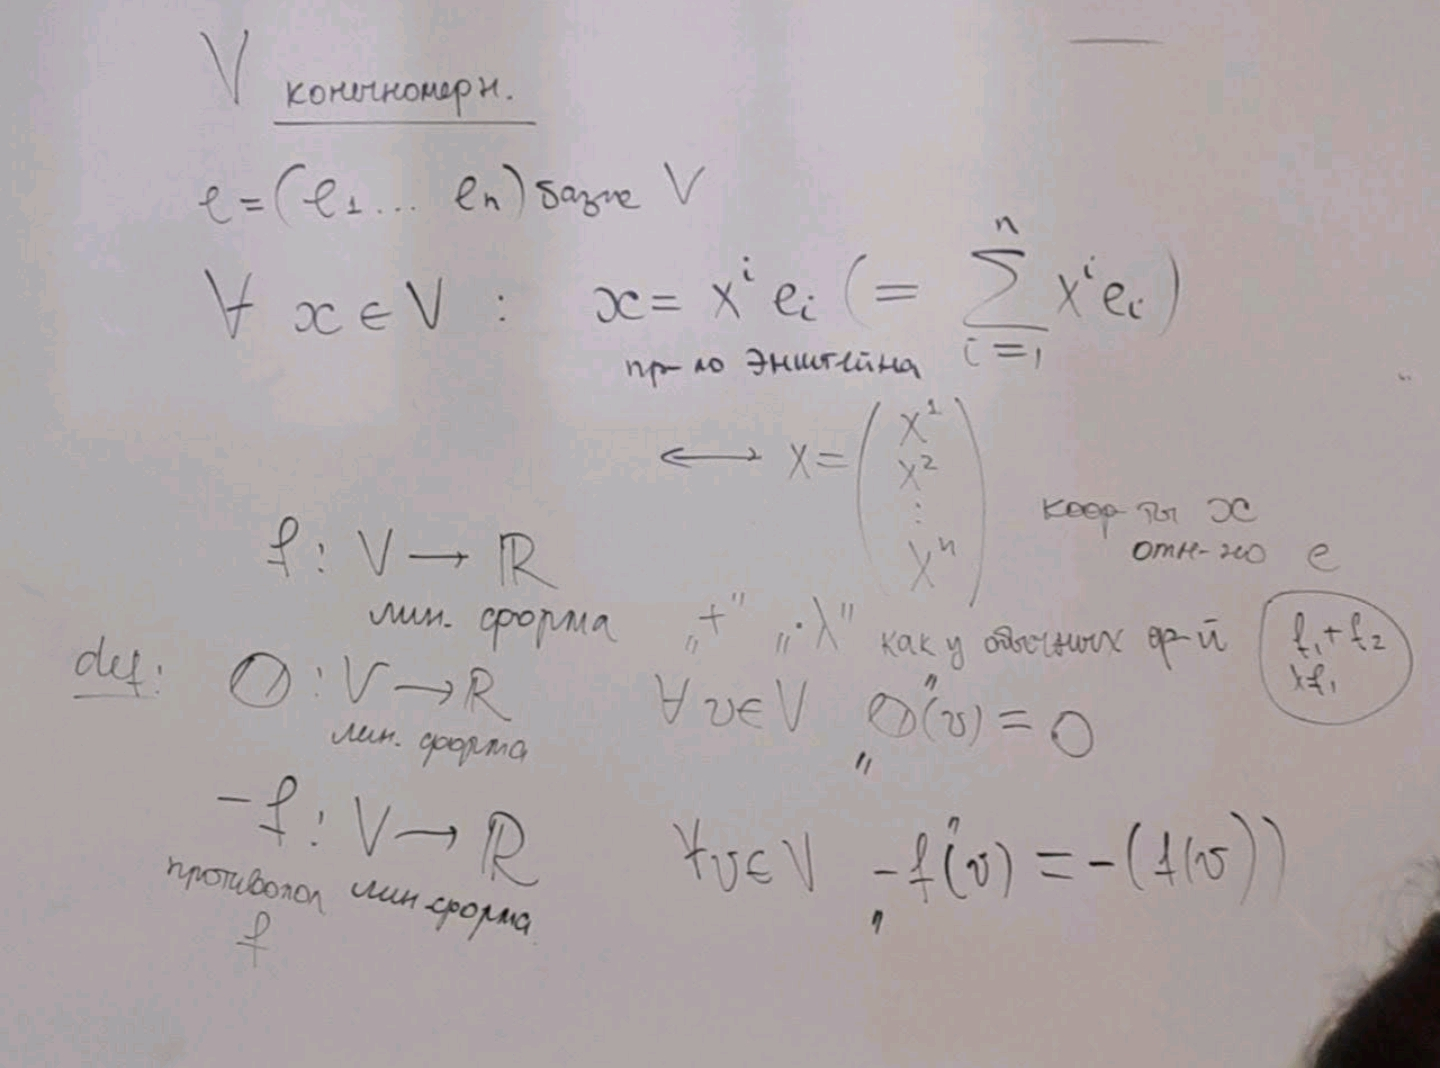
\includegraphics[width=0.93\textwidth]{kek2/kek2_00004}\n
	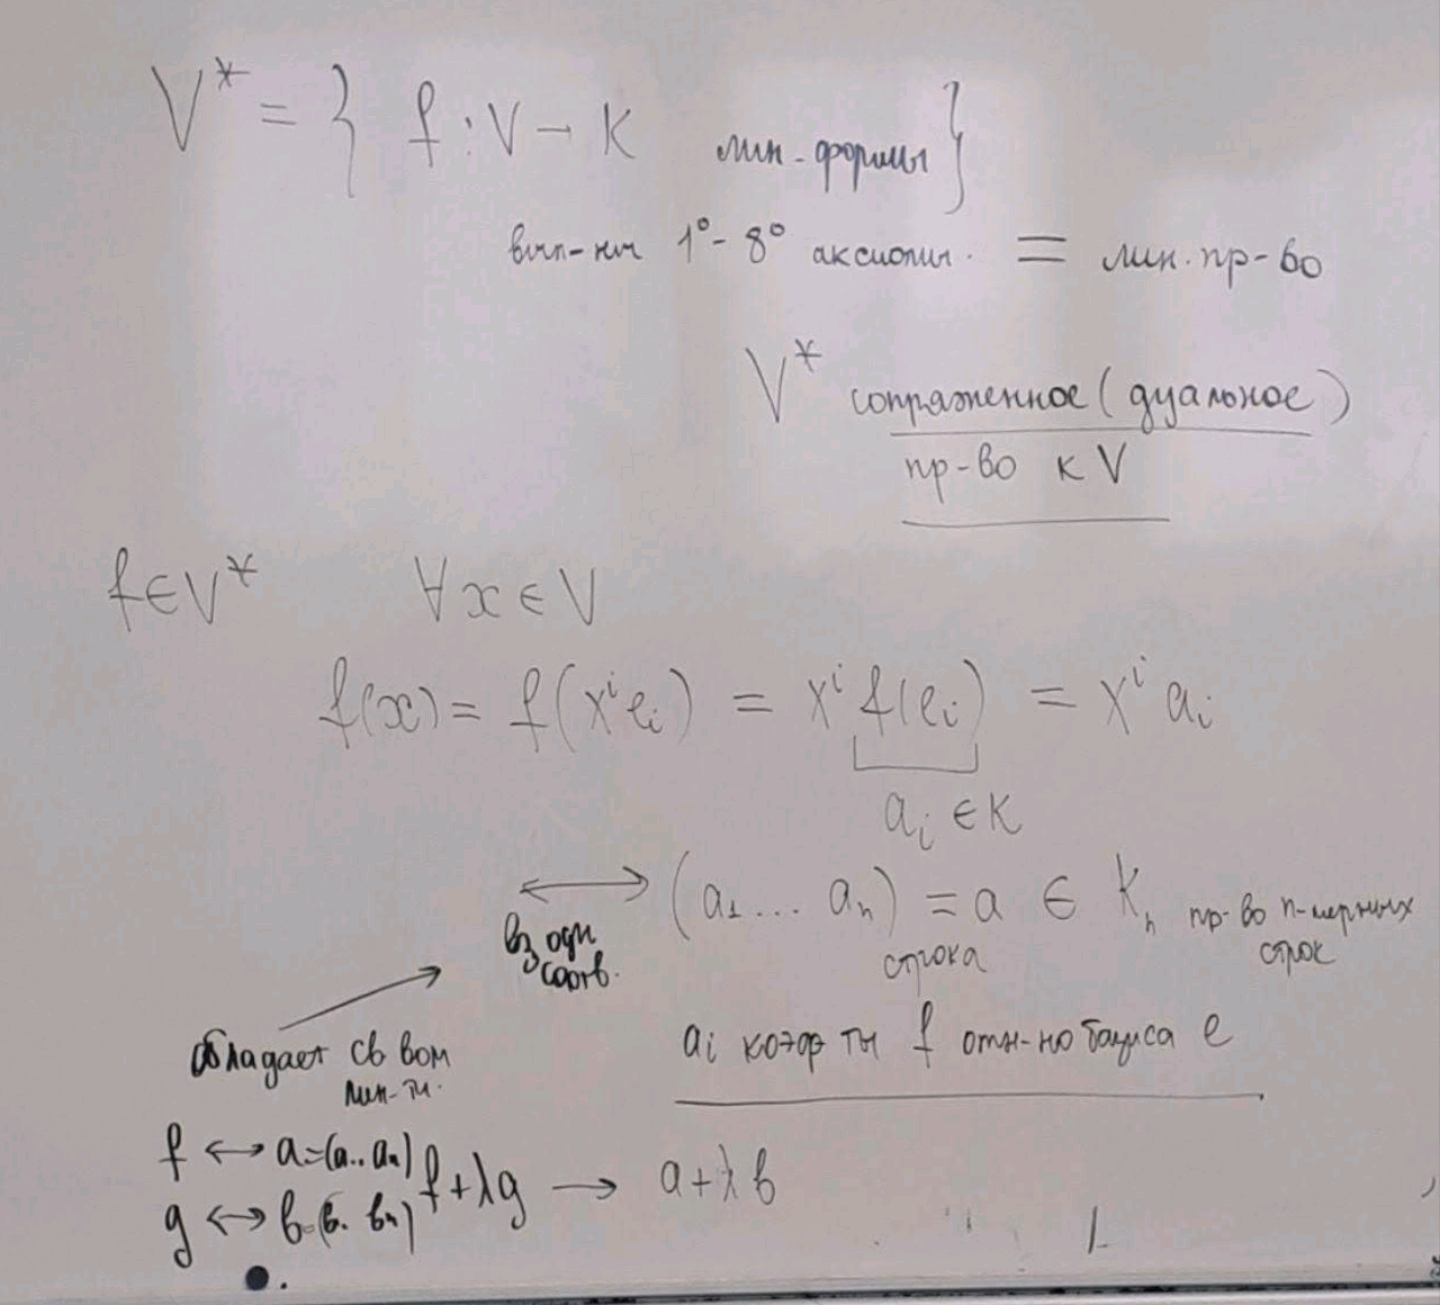
\includegraphics[width=\textwidth]{kek2/kek2_00005}\n
	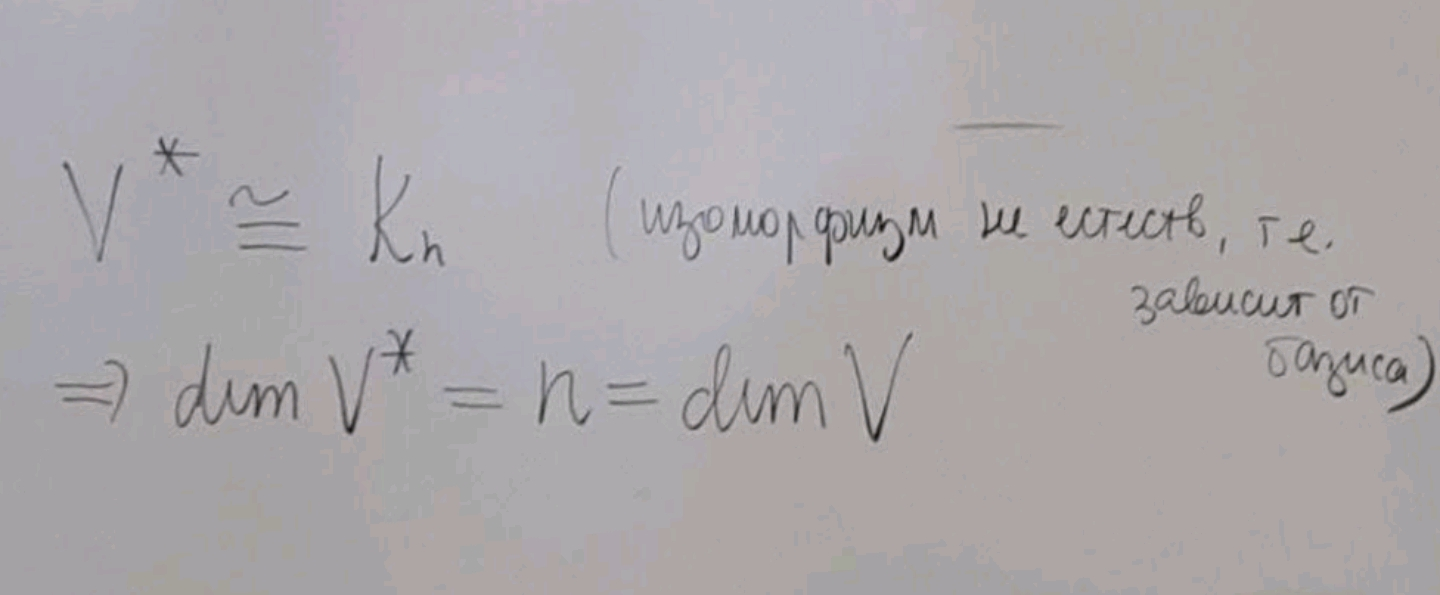
\includegraphics[width=\textwidth]{kek2/kek2_00006}
\end{document}